\documentclass[10pt]{article}

\usepackage[utf8]{inputenc}
\usepackage[T1]{fontenc}
\usepackage{amsmath}
\usepackage{mathtools}
\usepackage{amssymb}
\usepackage{graphicx}
%\usepackage[dvipsnames]{xcolor}
\usepackage{units}
%\usepackage{wrapfig}
%\usepackage{float}
%\usepackage{fancyhdr} %fancyheadings
\usepackage[margin=\parindent]{caption} %caption of figures
\usepackage{color}
\usepackage{enumerate}
\usepackage{xpatch}
\usepackage{parskip}
\usepackage{hyperref}
\usepackage{booktabs}

\usepackage{geometry}
\geometry{paperheight=238mm,paperwidth=168mm, left=10mm, top=8mm, right=10mm, bottom=16mm}

\usepackage[backend=biber, style=numeric-comp, sorting=none, hyperref=true, url=false, doi=false, backref=true, firstinits=true, isbn=false]{biblatex}
\newbibmacro{string+doi}[1]{%
  \iffieldundef{doi}{#1}{\href{http://dx.doi.org/\thefield{doi}}{#1}}}
\DeclareFieldFormat{title}{\usebibmacro{string+doi}{\mkbibemph{#1}}}
\DeclareFieldFormat[article]{title}{\usebibmacro{string+doi}{\mkbibquote{#1}}}

\hypersetup{colorlinks=true, linkcolor=my_blue, urlcolor=blue, citecolor=my_green}
\urlstyle{same}


\usepackage{tikz}
\usetikzlibrary{shapes.geometric, positioning, decorations.markings} 
\usetikzlibrary{arrows.meta, graphs, shapes.misc} 
\usetikzlibrary{calc}
\usetikzlibrary{backgrounds}

\bibliography{dps_theory.bib}

\graphicspath{{./}{pics/}}

\newcommand{\ket}[1]{| #1 \rangle}
\newcommand{\bra}[1]{\langle#1|}
\newcommand{\braket}[2]{\langle#1|#2\rangle}
\newcommand{\Tr}{\mathop{\mathrm{Tr}}\nolimits}




\definecolor{vq_green}{RGB}{0,235,210}
\definecolor{vq_blue}{RGB}{0,173,234}
\definecolor{my_blue}{RGB}{0,0,200}
\definecolor{my_green}{RGB}{0,200,0}
\definecolor{my_red}{RGB}{200,0,0}
\newcommand{\bl}[1]{\textcolor{my_blue}{#1}}
\newcommand{\me}[1]{\langle\colon{#1}\colon\rangle}

%\usepackage[automark,headsepline]{scrlayer-scrpage}

%\clearpairofpagestyles
%\cfoot[\pagemark]{\pagemark}
%\lehead{\headmark}
%\rohead{\headmark}
%\pagestyle{scrheadings}

\usepackage{enumitem}
\setlist{nolistsep}


\begin{document}

\title{FPGA work to be done}

\author{Veriqloud}

\date{}
\maketitle

%\vspace{-2cm}



\section{Context}
We have a prototype quantum key distribution system (QKD). We want to improve it's reliability and performance. 
We split this work into two projects: 
\begin{itemize}
    \item \textbf{Turnkey:} Migrate from Lattice ECP5 to Xilinx Artix Ultrascale+. 
        Keep optics and electronics.
    \item \textbf{Performance:} Change encoding to side-channel-secure scheme, increase pulse repetition. 
        Assemply and optics done by IDIL.\@ 
        FPGA code changes only slightly with respect to project Turnkey.
\end{itemize}


\section{Cards in the system}
See Fig.~\ref{fig:current_system} for an overview of the current system. The main modifications on this level for project Turnkey will be to
\begin{itemize}
    \item replace the FPGA board by the \href{https://opalkelly.com/products/xem8310/}{XEM8310} from OpalKelly.
    \item replace the NUC by a PC on a Mini-ITX motherboard and make it communicate over PCIe to the FPGA board. Remove FTDI Uart and USB.\@
    \item remove Eth at the FPGA level and route communication through PCIe.
    \item remove the RaspberryPi, plug the RNG into the PC and communicate the random numbers over PCIe.
\end{itemize}

\begin{figure}[!h]
    \centering
    \includegraphics[width=0.6\textwidth]{DUD.pdf}
    \caption{The current system. The \href{https://github.com/butterstick-fpga/butterstick-hardware}{Butterstick} is an open-source board around the Lattice ECP5 FPGA.}%
    \label{fig:current_system}
\end{figure}

New system system should look something like this:

\begin{tikzpicture}[font = \small]
    % top
    \node[align=center] (switch) at (-4,3) {Eth Switch\\Orolia\\White Rabbit};
    \node[align=center] (clock) at (0,3) {Clock\\ltc6951};
    \node[align=center] (dac) at (4,3) {DAC\\ad9152};
    % middle
    \node[align=center, fill=vq_blue!30] (fpga) at (0,0) {FPGA\\Xilinx Artix\\Ultrascale+\\\href{https://opalkelly.com/products/xem8310/}{XEM8310}}; 
    \node[align=center] (slow) at (4,0) {Slow\\DAC/ADC};
    \node[align=center] (pc) at (-4,0) {PC\\i7-12700T\\ASRock\\\href{https://www.asrock.com/MB/Intel/Z690M-ITXax/index.fr.asp#Specification}{Z690M-ITX/ax}};
    % bottom
    \node[align=center] (rng) at (-4,-3) {tRNG\\TectroLabs\\\href{https://tectrolabs.com/swiftrng-pro/}{SwiftRNG Pro}};
    \node[align=center] (jc) at (0,-3) {Jitter Cleaner\\Si5317};
    \node[align=center] (tdc) at (4,-3) {TDC\\AS6501};
    \node[align=center] (apd) at (4,-5) {APD\\\href{https://www.aureatechnology.com/en/products/oem-photon-counter.html}{Aurea SPD\_OEM\_NIR}};
    % connections
    \draw[->, font=\scriptsize] (switch) -- (clock) node[above, midway]{10MHz + 1PPS};
    \draw[<->, font=\scriptsize] (pc) -- (fpga) node[above, midway]{PCIe};
    \draw[->, font=\scriptsize] (rng) -- (pc) node[midway, above, sloped]{USB};
    \draw[->, font=\scriptsize] (fpga) -- (jc) node[midway, above, sloped]{5MHz};
    \draw[->, font=\scriptsize] (jc) -- (tdc) node[midway, above]{5MHz};
    \draw[<->, font=\scriptsize] (fpga) -- (slow) node[midway, above]{SPI};
    \draw[->, font=\scriptsize] (fpga) -- (dac) node[midway, sloped, above]{JESD205B};
    \draw[->, font=\scriptsize] (clock) -- (fpga) node[midway, sloped, above]{clk};
    \draw[->, font=\scriptsize] (clock) -- (dac) node[midway, above]{jesd\_clk};
    \draw[->, font=\scriptsize] (apd) -- (tdc) node[midway, right]{TTL pulse};
    \draw[->, font=\scriptsize] (tdc) -- (fpga) node[midway, above, sloped]{time stamp};
    \draw[<->, font=\scriptsize] (pc) -- (switch) node[midway, above, sloped]{Eth\_cc};
    \draw[<->, font=\scriptsize] (pc) -- ++(-3,0) node[midway, above]{Eth\_user};

    \begin{scope}[on background layer]
        \fill[fill=vq_green!20] (jc.south west) rectangle (slow.east|-dac.north);
    \end{scope}

\end{tikzpicture}

\section{Dataflow}

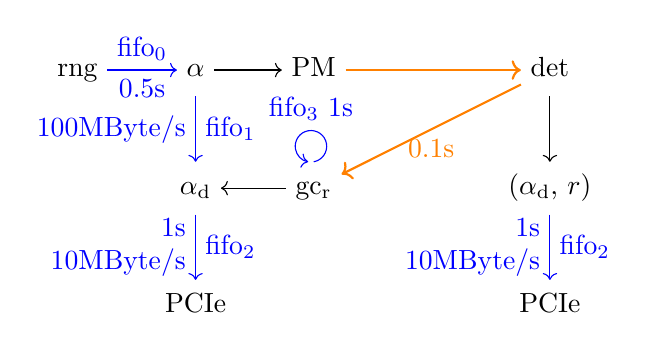
\begin{tikzpicture}[font = \normalsize, node distance=1.5cm, 
    ofast/.style={draw, black, fill=blue!30, minimum size=0.8cm, thin},
    osidechannel/.style={draw, black, fill=blue!30, minimum size=0.8cm, minimum width=1.2cm, thin},
    ofilter/.style={draw, black, fill=red!40, minimum size=0.8cm, thin},
    naked/.style={minimum size = 0},
    fiber/.style={orange, thick},
    fibera/.style={orange, thick, ->},
    fiberbg/.style={white, line width=5pt},
    fifo/.style={blue, ->},
    arrow/.style={->},
    ]

    \coordinate (dx) at (1.5,0);
    \coordinate (c1) at (4,1.5);
    \coordinate (c2) at (6,1.5);
    \coordinate (c3) at (8,1.5);

    \node(rng){\strut rng};
    \node(angle)[right of = rng]{\strut $\alpha$};
    \node(pm)[right of = angle]{\strut PM};
    \node(det)[right of = pm, node distance=3cm]{\strut det};
    \node(gc)[below of = pm]{\strut gc$_\textnormal{r}$};
    \node(dangle)[below of = angle]{\strut $\alpha_\textnormal{d}$};
    \node(dangle2)[below of = det]{\strut ({\strut $\alpha_\textnormal{d}$}, $r$)};
    \node(PCIe)[below of = dangle]{\strut PCIe};
    \node(PCIe2)[below of = dangle2]{\strut PCIe};

    \draw[fifo](rng) -- (angle) node[above, pos=0.5]{fifo$_0$} node[below,pos=0.5]{0.5s};
    \draw[fifo](angle) -- (dangle) node[right, pos=0.5]{fifo$_1$} node[left, pos=0.5, align=right]{100MByte/s};
    \draw[fifo](dangle) -- (PCIe) node[right, pos=0.5]{fifo$_2$} node[left, pos=0.5, align=right]{1s\\10MByte/s};
    \draw[arrow](det) -- (dangle2) ;
    \draw[fifo](dangle2) -- (PCIe2) node[right, pos=0.5]{fifo$_2$} node[left, pos=0.5, align=right]{1s\\10MByte/s};
    
    \draw[fibera](det) -- (gc) node[below, pos=0.5]{0.1s};
    \draw[arrow](angle) -- (pm);
    \draw[arrow](gc) -- (dangle);
    \draw[fibera](pm) -- (det);

    %\draw[arrow,fifo] (gc.north)++(0.05,0) to[out=30, in=0] ++(-0.05,0.3) node[above]{filo$_4$ 1s} to[out=180, in=150] +(-0.05,-0.3);
    \draw[arrow,fifo] (gc.north) arc (-80:260:0.2) node[above, pos=0.5]{fifo$_3$ 1s};

    
    

\end{tikzpicture}

\section{User Interface}

As of ETSI standards, there are four users at the top level:
\begin{itemize}
    \item Administrator (us, the manufacturer)
    \item Maintainer (customer)
    \item Auditor (no idea who this is)
    \item Key Requestor (program running on customer machine)
\end{itemize}

From the FPGA point of view, we are at a lower level. For us there are two users who interact independently.
\begin{itemize}
    \item post processing
    \item control
\end{itemize}


\subsection{Post processing functions}

\begin{tabular}{l l}
%    \toprule 
    {\tt get\_current\_gc} & get current global counter \\
    {\tt start\_at\_gc} & start running  \\
    {\tt read\_angles} & download angles \\
    {\tt idle} & do nothing \\
    {\tt get\_count\_rates} & get current click rates \\
    {\tt write\_config} & update config from a file (angles, bias, VCA, gates, \dots) \\
%    \bottomrule 
\end{tabular}

\subsection{Control functions}

\begin{tabular}{l l}
%    \toprule 
    {\tt reset} & reset FPGA \\
    {\tt sync} & sync at next PPS  \\
    {\tt jc\_comm} & interact with jitter cleaner \\
    {\tt tdc\_comm} & interact with tdc \\
    {\tt ad\_comm} & interact with clock chip \\
    {\tt ltc\_comm} & interact with DAC \\
    {\tt tdc\_rcv\_time} & download time of events \\
    {\tt tdc\_rcv\_click} & download result of events \\
    {\tt dac\_seq} & write periodic sequence to FPGA \\
    {\tt get\_count\_rates} & get current click rates \\
    {\tt write\_config} & update config from a file (angles, bias, VCA, gates, \dots) \\
%    \bottomrule 
\end{tabular}

%\printbibliography%


\section{Deliverables}

Make the system work without hardware issues.

\section{Calibration procedure}

\subsection{Find gates}

\begin{itemize}
    \item Alice sends double pulses and sweeps the phases (to get equally high peaks in the arrival time histogram). 
    \item Bob download the arrival times modulo qubit distance
    \item Bob (in software) searches for the peaks and writes offset and time to config/gates.json
    \item Bob writes config/gates.json to FPGA
\end{itemize}

\subsection{Fine tune phase-modulator time offset}

\begin{itemize}
    \item Bob turns on feedback.
    \item Bob puts two different values on the phase modulator for various delays and downloads the click statistics
    \item Bob (in software) finds the best delay and writes to config/delays.json
    \item Bob takes a sine measurement: 64 periodic sweep on the phase modulator. From this, the four angles are calculated and written to config/angles.json
    \item Repeat for Alice and Charlies
\end{itemize}

\subsection{Find delay}

\begin{itemize}
    \item run periodic patterns on the phase modulator. E.g.\ alpha0 for the first point and alpha1 for the rest.
    \item download the click data and find alpha0 and write appropriate delay to config/delays.json
    \item repeat for everybody
\end{itemize}

\subsection{Check qber}

\begin{itemize}
    \item run pseudo random sequency of BB84 angles for individuals or on the entire qline.
    \item download click data and check qber.
\end{itemize}

\subsection{Optimize polarization}

\begin{itemize}
    \item in parallel to other things: try to increase the count rates by changing polarization. Do this for every player one after the other
\end{itemize}

\subsection{Optimize bias}

\begin{itemize}
    \item from the qber, optimize bias.
\end{itemize}

\section{Error signals}

\begin{itemize}
    \item count rates drop/rise
    \item dac or clock out of lock
\end{itemize}

\section{Hardware tests}

\subsection{TDC readout}

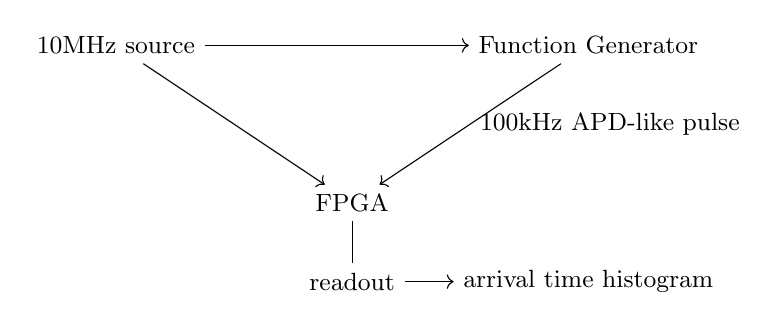
\begin{tikzpicture}[font = \small]
    \node (s) at (0,0) {10MHz source};
    \node (fg) at (6,0) {Function Generator};
    \node (fpga) at (3,-2) {FPGA};
    \node (pc) at (3,-3) {readout};
    \node (hist) at (6,-3) {arrival time histogram};

    \draw[->] (s) --  (fg);
    \draw[->] (s) --  (fpga);
    \draw[->] (fg) -- (fpga) node[midway, right]{100kHz APD-like pulse};
    \draw[->] (fpga) -- (pc) -- (hist);

\end{tikzpicture}

\subsection{Gates}

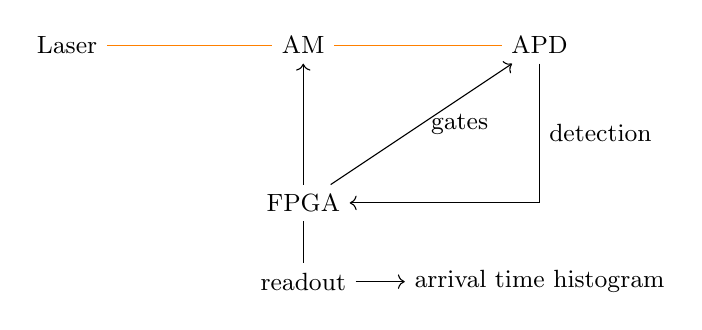
\begin{tikzpicture}[font = \small]
    \node (laser) at (0,0) {Laser};
    \node (am) at (3,0) {AM};
    \node (apd) at (6,0) {APD};
    \node (fpga) at (3,-2) {FPGA};
    
    \node (pc) at (3,-3) {readout};
    \node (hist) at (6,-3) {arrival time histogram};
    
    \draw[orange] (laser) -- (am) -- (apd);

    \draw[->] (fpga) -- (pc) -- (hist);
    \draw[->] (fpga) -- (am);
    \draw[->] (fpga) -- (apd) node[midway, right]{gates};
    \draw[->] (apd) |- (fpga) node[near start, right]{detection};
\end{tikzpicture}

\begin{itemize}
    \item Verify through APD UI that it receives the gates at the desired frequency. 
    \item Generate double pulses below single-photon level. Put onto APD. 
    \item plot arrival time histograms, position the gates and verify that the peaks look as expected and the count rates make sense.
\end{itemize}


\subsection{Interference visibility}

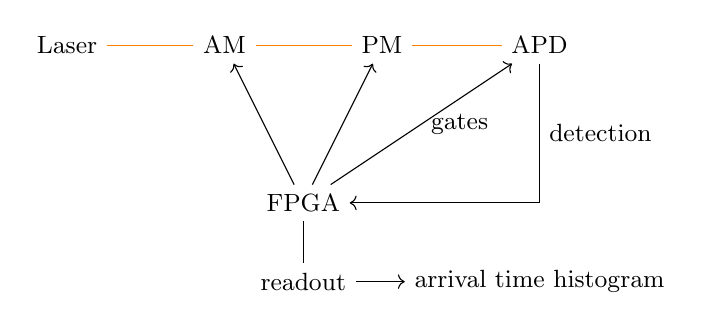
\begin{tikzpicture}[font = \small]
    \node (laser) at (0,0) {Laser};
    \node (am) at (2,0) {AM};
    \node (pm) at (4,0) {PM};
    \node (apd) at (6,0) {APD};
    \node (fpga) at (3,-2) {FPGA};
    
    \node (pc) at (3,-3) {readout};
    \node (hist) at (6,-3) {arrival time histogram};
    
    \draw[orange] (laser) -- (am) -- (pm) -- (apd);

    \draw[->] (fpga) -- (pc) -- (hist);
    \draw[->] (fpga) -- (am);
    \draw[->] (fpga) -- (pm);
    \draw[->] (fpga) -- (apd) node[midway, right]{gates};
    \draw[->] (apd) |- (fpga) node[near start, right]{detection};
\end{tikzpicture}

\begin{itemize}
    \item Sweep phases and plot the sin histogram. 
    \item Turn feedback on, select proper angles and measure the qber. 
\end{itemize}

\subsection{Sync between Alice and Bob}

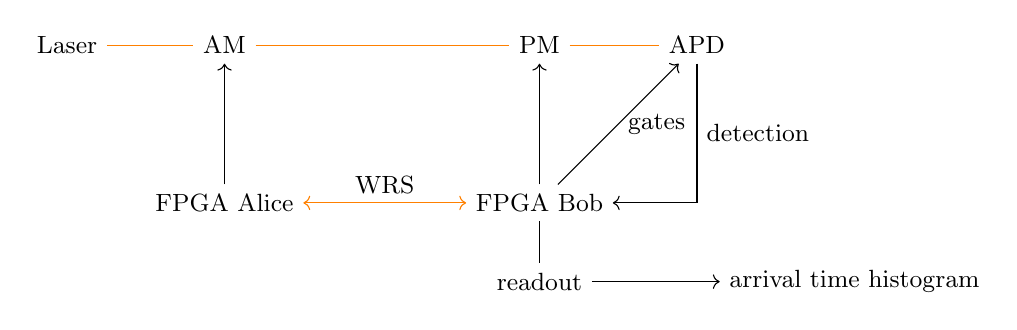
\begin{tikzpicture}[font = \small]
    \node (laser) at (-2,0) {Laser};
    \node (am) at (0,0) {AM};
    \node (pm) at (4,0) {PM};
    \node (apd) at (6,0) {APD};
    \node (fpgaa) at (0,-2) {FPGA Alice};
    \node (fpgab) at (4,-2) {FPGA Bob};
    
    \node (pc) at (4,-3) {readout};
    \node (hist) at (8,-3) {arrival time histogram};
    
    \draw[orange] (laser) -- (am) -- (pm) -- (apd);

    \draw[->] (fpgab) -- (pc) -- (hist);
    \draw[->] (fpgaa) -- (am);
    \draw[->] (fpgab) -- (pm);
    \draw[->] (fpgab) -- (apd) node[midway, right]{gates};
    \draw[->] (apd) |- (fpgab) node[near start, right]{detection};
    \draw[<->, orange] (fpgaa) -- (fpgab) node[black, midway, above] {WRS};
\end{tikzpicture}

\subsection{Communication and dataflow between players}

\subsection{Automated calibration procedure}

\subsection{QKD}






\end{document}

















